%! TEX root = ../main.tex

\chapter{Interpolation and Growth Conditions}~\label{ch:interpolation-gc}

Interpolation is a technique from numerical analysis where a function is approximated by exactly fitting a sample of its evaluations using a tractable class of approximators. 
This class is often piece-wise linear, piece-wise cubic, or polynomial, but can also be non-parametric. 
Even over-parameterized neural networks can be used, assuming it is possible to solve the resulting non-convex optimization problem. 
This is because the defining aspect of interpolation methods is not the choice of approximating function, but that the approximation attains the \emph{true} function value at all points in the sample.


This basic notion of interpolation can be directly carried over to supervised machine learning.  
The regression case is nearly identical --- intuitively, a model interpolates a set of training examples if it predicts exactly the true target for each example. 
The analogy to numerical analysis is complete if we assume that the data are generated by an underlying deterministic mapping.
For classification problems, interpolation can be defined in two obvious ways. 
We might say a model satisfies interpolation if it predicts the correct class for each training example, or alternatively, if it attains zero loss for all training examples.  
The latter interpretation is dependent on the choice of objective function and starts to hint at the role of interpolation in optimization.
Note that in the regression example, the two notions of interpolation coincide for the natural choice of squared loss on all examples.

These intuitive definitions for interpolation mean approximately the same thing: ``to fit the data exactly''. 
While this agrees with the spirit of the methodology and broader scientific usage of the term, a rigorous definition is necessary to analyze the complexity of first-order optimizers under interpolation. 
This chapter formalizes interpolation in the context of stochastic optimization. 
In particular, we do the following:
\begin{enumerate}
    \item Define the concept of a \ac{SFO} \oracle{} and propose a new Lipschitz-smoothness property for \acp{SFO}, which we call individually-smoothness. 
    \item Give three specific definitions of interpolation in the context of a \acl{SFO} and objective function pair \( \rbr{f, \oracle{}} \). 
    These are the first definitions applicable to the general stochastic setting.
    \item Characterize the relationships between the three models of interpolation as well as connections to strong and weak growth. 
In particular, we show that interpolation implies weak growth if \oracle{} is individually-smooth; this relaxes existing sufficient conditions, which further assume \( f \) is convex and finite-sum~\citep{vaswani2019fast}. 
\end{enumerate}
We begin with the discussion of stochastic oracles.

\section{Stochastic Oracles}~\label{sec:stochastic-oracles}

The defining feature of stochastic optimization algorithms is that they cannot directly access the value or gradient of the objective function \( f \).
Instead, they obtain noisy function and gradient evaluations through a \ac{SFO}  \oracle. 
At each iteration \( k \), \oracle{} outputs a stochastic function \( f(\w, \zk) \) and gradient \( \grad(\w, \zk) \) at query point \( \w \), where \( \zk \) is a random variable with distribution \( \mu_k \) supported on \( \calZ_k \subseteq \R^m \), \( m > 0 \).%%
\footnote{It will be sufficient to treat the measure \( \mu_k \) as a prob.\ density function \( p_k \) for nearly all of our purposes.}
We assume that \( f(\w, \cdot) \) is a deterministic Borel function, meaning the stochasticity in \( f(\w, \zk) \) stems only from the random variable \( \zk \).
Similarly, \( \grad(\w, \cdot) \) is taken to be a deterministic Borel function related to \( f(\w, \cdot) \) through the standard differentiation operator,
\[ \grad(\w, \cdot) = \sbr{\frac{\partial}{\partial_{w_1}} f(\w, \cdot), \ldots, \frac{\partial}{\partial_{w_d}} f(\w, \cdot)}^\top. \]
Unless stated otherwise, the oracle outputs are always taken to be unbiased, implying that 
\begin{align*}
    \E_{\zk} \sbr{f(\w, \zk)} = f(\w) \quad \text{and} \quad \Ek \sbr{\grad(\w, \zk)} = \grad(\w), 
\end{align*}
for all \( k \).

The definition of \oracle{} is non-stationary in the sense that it allows the distributions \( \mu_k \) and their support \( \calZ_k \) to change across iterations.
As such, it will be necessary to refer to the support of the entire stochastic process \( \seq{\zk} \), 
\[ \calZ = \bigcup_{k\in \bbN} \calZ_k. \]
For simplicity, \( \calZ \) is called the support of \oracle{}. 
Note that a statement which holds point-wise over \( \calZ \) holds almost-surely for all \( \zk \).
These two requirements are equivalent, since (by definition) every \( \z \in \calZ \) is in the support of some \( \mu_k \).
We will make use of this less cumbersome notation. 

Some results will further require that the stochastic function \( f(\cdot, \zk) \) is Lipschitz-smooth for all outcomes in \( \calZ \).
In this case, we say \oracle{} satisfies \emph{individual smoothness} with parameter \( \Lmax \).
\begin{restatable}[Individual Smoothness]{definition}{individuallySmooth}~\label{def:individually-smooth}
    An \ac{SFO} \oracle{} is called \( \Lmax \) individually-smooth if the stochastic gradient mapping \( \w \mapsto \grad(\w, \z) \) is \( L_{\z} \)-Lipschitz with \( L_{\z} \leq \Lmax \) for all \( \z \in \calZ \).
\end{restatable}
\noindent Individual smoothness implies the quadratic upper bound
\[ f(v, \z) \leq f(\w, \z) + \abr{\grad(\w, \z), v - \w} + \frac{\Lmax}{2}\norm{v - \w}^2 \quad \forall v, \w \in \R^d, \]
holds point-wise over \( \calZ \) and thus almost-surely for each \( \zk \).
Note that the existence of an \( \Lmax \) individually-smooth, unbiased \ac{SFO} for \( f \) implies that \( f \) is \( L \)-smooth with \( L \leq \Lmax \) as an immediately corollary.
\begin{restatable}{corollary}{indSmoothToSmooth}~\label{cor:ind-smooth-to-smooth}
    Let \( f : \R^d \rightarrow \R \) be a differentiable function.  
    If there exists an unbiased, \( \Lmax \) individually-smooth \ac{SFO} \oracle{} for \( f \), then \( f \) is \( L \)-smooth with \( L \leq \Lmax \).
    Alternatively, if \( \oracle{} \) is biased but the support \( \calZ \) is finite and the partial derivatives \( \frac{\partial}{\partial w_j} f(\w, \z) \) are finite for each \( z \in \calZ \), then \( \Ek \sbr{f(\cdot, \zk)} \) is \( \Lmax \)-smooth for all \( k \). 
\end{restatable}
\noindent See \autoref{app:stochastic-oracles} for proof. 
In several cases, we will also make use of individual strong-convexity.
\begin{restatable}[Individual Strong-Convexity]{definition}{individuallySC}~\label{def:individually-sc}
    A \ac{SFO} \oracle{} is called \( \mumax \) individually-strongly-convex if the function \( f(\cdot, \z) \) is \( \mu_{\z} \)-strongly-convex with \( \mu_{\z} \leq \mumax \) for all \( \z \in \calZ \).
    If \( \mumax = 0 \), then we say \oracle{} is individually-convex.
\end{restatable}

Individually-smooth oracles are wide-spread throughout machine learning in the form of finite-sum functions. 
Recall that finite-sum functions are a particular class of structured optimization problem where the objective \( f \) is the sum of \( n \) sub-functions. 
The following example demonstrates individual smoothness in the context of least-squares regression. 
\begin{example}[Least Squares Regression: Individual Smoothness]\label{example:ls-ind-smooth}
    The classic least-squares regression problem
    \[ \wopt = \argmin \frac{1}{n} \sum_{i=1}^n \rbr{\abr{w, x_i} - y_i}^2, \]
    has a finite-sum structure with \( f_i(\w) =  \rbr{\abr{w, x_i} - y_i}^2\).
    The mini-batch \ac{SFO} uniformly sub-samples \( b \leq n \) examples to obtain the following function and gradient estimators:
    \[ f(\w, \z) = \frac{1}{b} \sum_{i \in \z}  \rbr{\abr{w, x_i} - y_i}^2 \; \text{ and } \; \grad(\w, \z) = \frac{1}{b} \sum_{i \in \z} 2 \rbr{\abr{w, x_i} - y_i} x_i, \]
    where \( \z \in \calZ = \cbr{ A \subseteq \cbr{1, \dots, n} : |A| = b } \) is the set of sampled indices.
    Notice that \( f(\cdot, \z) \) is convex and \( L_z \)-smooth with \( L_z = \frac{2}{b} \norm{\sum_{i \in \z} x_z x_z^\top}_\text{op}^2 \), where $\norm{\cdot}_{\text{op}}$ is the operator norm.
    This implies \oracle{} is individually-convex and \( \Lmax \) individually-smooth with \( \Lmax \leq 2 \max_{i \in [n]} \norm{x_i}^2 \). 
\end{example}

\autoref{example:ls-ind-smooth} illustrates the \emph{mini-batch} oracle commonly used in machine learning.
The mini-batch oracle is unbiased, simple to compute, and by far the most common \ac{SFO} in machine learning. 
If the sub-functions \( f_i \) are each individually \( L_i \)-smooth, then the mini-batch \ac{SFO} satisfies individual-smoothness with \( \Lmax = \max_{i\in [n]} L_i \).
We call general \acp{SFO} individually-smooth specifically to invite comparison with this natural property of the mini-batch oracle. 


\section{Interpolation}~\label{sec:interpolation}

Now we formalize interpolation in the context of stochastic optimization problems.
Unlike previous work, we consider general \acp{SFO} and do not require \( f \) to be finite-sum or \oracle{} to be the mini-batch oracle (cf. \citet{vaswani2019fast} or \citet{bassily2018exponential}).
Instead, three different notions of interpolation are developed as a joint property of the objective and oracle. 
As with individual smoothness, interpolation is shown to have a simple realization for finite-sum functions that satisfies the intuition previously developed for machine learning problems. 

The basic requirement of interpolation is that the oracle outputs \( f(\cdot, \z) \) and \( \grad(\cdot, \z) \) resemble the true function at key target points.  
The axes of variation in the definitions to follow are (a) the specific target points and (b) the type of ``matching'' required.
Unlike classic interpolation, matching here refers to mutual optimality or mutual stationarity, rather than a requirement for equal function values; 
enforcing \( f(\wopt) = f(\wopt, \z) \) may not be useful from an optimization perspective, since \( \grad(\wopt, \z) \) could be non-zero.
The three definitions are as follows:

\begin{definition}[Interpolation: Minimizers]\label{def:interpolation-minima}
    A function-oracle pair \( (f, \oracle{}) \) satisfies minimizer interpolation if for all \( \z \in \calZ \),
    \[ f(\w') \leq f(\w) \; \forall \w \in \R^d \implies f(\w', \z) \leq f(\w, \z) \; \forall \w \in \R^d.  \]
\end{definition}
\begin{definition}[Interpolation: Stationary Points]\label{def:interpolation-gradients}
    A function-oracle pair \( (f, \oracle{}) \) satisfies stationary-point interpolation if for all \( \z \in \calZ \),
    \[ \grad(\w') = 0 \implies \grad(\w', \z) = 0. \]
\end{definition}
\begin{definition}[Interpolation: Mixed]\label{def:interpolation-mixed}
    A function-oracle pair \( (f, \oracle{}) \) satisfies mixed interpolation if for all \( \z \in \calZ \),
    \[ f(\w') \leq f(\w) \; \forall \w \in \R^d \implies \grad(\w', \z) = 0. \]
\end{definition}
In words, \autoref{def:interpolation-minima} states that global minimizers of the objective \( f \) must be global minimizers of the stochastic functions given by the \ac{SFO} at every iteration \( k \).
In contrast, \autoref{def:interpolation-gradients} puts the same requirement on stationary points of \( f \), while \autoref{def:interpolation-mixed} merely demands that minimizers of \( f \) are stationary points of \( f(\cdot, \z) \) for all outcomes \( \z \).

For general functions and \acp{SFO}, the relationship between these models of interpolation is limited to the following: minimizer interpolation and stationary-point interpolation are stronger than mixed interpolation. 
However, all three definitions are equivalent when \( f \) and \( f(\cdot, \z) \) are invex for all \( z \in \calZ \).
This is stated in the following lemma.
\begin{restatable}{lemma}{interpRelationships}~\label{thm:interp-relationships}
    Let \( \rbr{f, \oracle{}} \) be an arbitrary function-\ac{SFO} pair. 
    Then only the following relationships hold between models of interpolation:
    \begin{align*}
        \text{Minimizer Interpolation} \; (\autoref{def:interpolation-minima}) &\implies \; \text{Mixed Interpolation} \; (\autoref{def:interpolation-mixed})\\
                                                                               & \text{and} &\\
        \text{Stationary-Point Interpolation} \; (\autoref{def:interpolation-gradients}) &\implies \; \text{Mixed Interpolation} \; (\autoref{def:interpolation-mixed}).
    \end{align*}
    However, if \( f \) is invex and \oracle{} is such that \( f(\cdot, \z) \) is invex for all \( \z \in \calZ \), then minimizer, stationary-point, and mixed interpolation are equivalent.
\end{restatable}
\noindent This result follows immediately from first-order optimality conditions and the equivalence of stationary points and global minimizers for invex functions.
For completeness, a short proof with counter-examples for the implications which do not hold is given in \autoref{app:interpolation-gc}.


\begin{figure}[t]
    \centering
    %% Demonstration of different definitions of interpolation.

\pgfplotsset{
    compat=1.5.1,
    oracle/.style={color=red, style=dashed, line width=1.5pt},
    objective/.style={color=black, style=solid, line width=1.5pt},
}

\tikzset{
    font={\fontsize{18pt}{12}\selectfont}},
}

\begin{figure}[]
    \centering
    \begin{tikzpicture}[scale=0.75, font size=50pt,
          declare function={
            objective(\x)=      (\x<=-1) * (2*\x*\x + 6*\x + 4)    +
            and(\x>-1, \x<=1) * (\x + 5 - pow(\x,3) - 5*\x*\x) / 4 +
                                (\x>1) * (\x*\x - 5*\x + 4); 
            oracle1(\x)=         (pow(\x - 2.5, 2) / 2 - 3.25);
          }
        ]
        \begin{axis}[
          axis x line=none, axis y line=none,
          ymin=-5, ymax=5, ytick={-5,...,5}, ylabel=$y$,
          xmin=-5, xmax=7, xtick={-5,...,7}, xlabel=$x$,
        ]
        \addplot[domain=-5:7, samples=100, objective]{objective(x)};
        \addplot[domain=-5:7, samples=100, oracle]{oracle1(x)};
        
        %% point labels
        \node[label={90:$\wopt$},circle,fill,inner sep=2pt] at (axis cs:2.5,-2.25) {};
        %% function labels
        \node[label={180:$f(\w)$}] at (axis cs:-2.4,2) {};
        \node[label={180:$f(\w, \z)$}] at (axis cs:1.25,-2.5) {};
        %% plot label
        \node[label={90:Minimizer}] at (axis cs:1,-5.2) {};
        \end{axis}
    \end{tikzpicture}%
    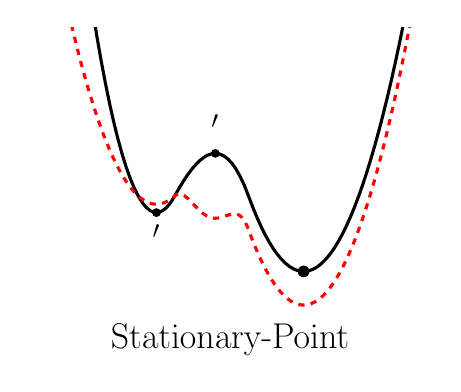
\begin{tikzpicture}[scale=0.75,
          declare function={
            objective(\x)=      (\x<=-1) * (2*\x*\x + 6*\x + 4)    +
            and(\x>-1, \x<=1) * (\x + 5 - pow(\x,3) - 5*\x*\x) / 4 +
                                (\x>1) * (\x*\x - 5*\x + 4); 
            oracle1(\x)=        (\x<=-1) * (pow(x + 1.5, 2))   +
            and(\x>-1, \x<=1) * (-305*pow(\x, 4)/264- 1*pow(\x, 3)/4 + 173*pow(\x,2)/132 - 1*\x/4 - 107/264) +
                                (\x>1) * (pow(x - 2.5, 2) - 3) - 0.25; 
          }
        ]
        \begin{axis}[
          axis x line=none, axis y line=none,
          ymin=-5, ymax=5, ytick={-5,...,5}, ylabel=$y$,
          xmin=-5, xmax=6, xtick={-5,...,6}, xlabel=$x$,
        ]
        \addplot[domain=-5:6, samples=100, objective]{objective(x)};
        \addplot[domain=-5:6, samples=200, oracle]{oracle1(x)};
        
        %% point labels
        \node[label={90:$\wopt$},circle,fill,inner sep=2pt] at (axis cs:2.5,-2.25) {};
        \node[label={90:$\w'$},circle,fill,inner sep=1.5pt] at (axis cs:0.1,1.262) {};
        \node[label={270:$\w'$},circle,fill,inner sep=1.5pt] at (axis cs:-1.5,-0.5) {};
        %% function labels
        %\node[label={0:$f(\w)$}] at (axis cs:-2.6,2.5) {};
        %\node[label={180:$f(\w, \z)$}] at (axis cs:1.25,-2.5) {};
        %% plot label
        \node[label={90:Stationary-Point}] at (axis cs:0.5,-5.2) {};
        \end{axis}
    \end{tikzpicture}%
    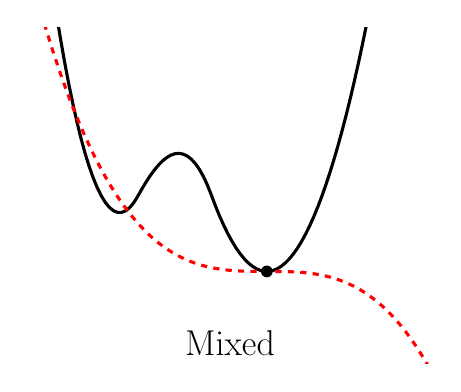
\begin{tikzpicture}[scale=0.75,
          declare function={
            objective(\x)=      (\x<=-1) * (2*\x*\x + 6*\x + 4)    +
            and(\x>-1, \x<=1) * (\x + 5 - pow(\x,3) - 5*\x*\x) / 4 +
                                (\x>1) * (\x*\x - 5*\x + 4); 
            oracle1(\x)=        -(1/30)*pow(x-2.5,3) - 2.25; 
          }
        ]
        \begin{axis}[
          axis x line=none, axis y line=none,
          ymin=-5, ymax=5, ytick={-5,...,5}, ylabel=$y$,
          xmin=-4, xmax=7, xtick={-5,...,7}, xlabel=$x$,
        ]
        \addplot[domain=-4:7, samples=100, objective]{objective(x)};
        \addplot[domain=-4:7, samples=200, oracle]{oracle1(x)};
        
        %% point labels
        \node[label={90:$\wopt$},circle,fill,inner sep=2pt] at (axis cs:2.5,-2.25) {};
        %% function labels
        %\node[label={0:$f(\w)$}] at (axis cs:-2.6,2.5) {};
        %\node[label={180:$f(\w, \z)$}] at (axis cs:1.25,-2.5) {};
        %% plot label
        \node[label={90:Mixed}] at (axis cs:1.5,-5.2) {};
        \end{axis}
    \end{tikzpicture}
    \caption{Differences in interpolation definitions in the finite-sum setting.}%
    \label{fig:interpolation-types}
\end{figure}


    \caption[Illustration of oracle samples satisfying different models of interpolation.]%
            {Oracle samples satisfying the three different models of interpolation for the same non-convex function.
             The dashed red-line is the graph of \( f(\w, \z) \) for a single, fixed \( \z \in \calZ \).
             Stationary-points are denoted as \( w' \), while the global minimizer is marked as \( \wopt \).
             Note that \( f(\w, \z) \) is permitted to have many ``extra'' stationary points when \oracle{} satisfies stationary-point interpolation.
         Similarly, mixed interpolation does not prevent \( f(\w, \z) \) from being unbounded below.}%
\label{fig:interpolation-types}
\end{figure}

Let us return to the finite-sum setting and mini-batch oracle to better understand the three definitions of interpolation.
In particular, let \( f \) and \oracle{} be such that
\[ f(\w) =  \frac{1}{n} \sum_{i=1}^{n} f_i(\w), \quad f(\w, \zk) = f_{\zk}(\w), \quad \grad(\w, \zk) = \grad_{\zk}(\w),  \]
where \( \mu_k \) is a uniform distribution over the support set \( \calZ = \cbr{1, \ldots, n} \).
The function-oracle pair \( \rbr{f, \oracle{}} \) satisfy minimizer interpolation if the individual functions \( f_i \) are globally minimized at every global minimum of \( f \).
The differences between minimizer and stationary-point interpolation are readily apparent for finite-sums of non-convex functions, as shown in \autoref{fig:interpolation-types}.
The following example further narrows this to least-squares regression, where interpolation implies the entire training set can be fit exactly.
\begin{example}[Least Squares Regression: Interpolation]\label{example:ls-interpolation}
    Consider the least-squares problem 
    \[ \wopt = \argmin \frac{1}{n} \sum_{i=1}^n \rbr{\abr{w, x_i} - y_i}^2, \]
    with individually-smooth and convex mini-batch oracle
    \[ f(\w, \z) = \frac{1}{|\z|} \sum_{i \in \z}  \rbr{\abr{w, x_i} - y_i}^2 \; \text{ and } \; \grad(\w, \z) = \frac{1}{|\z|} \sum_{i \in \z} 2 \rbr{\abr{w, x_i} - y_i} x_i. \]
    The stochastic functions \( f(\cdot, \z) \) are invex, as is \( f \), meaning minimizer, stationary-point, and mixed interpolation are equivalent. 
    If \( \rbr{f, \oracle} \) satisfies minimizer interpolation, then first-order optimality implies 
    \[  2 \rbr{\abr{\wopt, x_i} - y_i} x_i = 0 \quad \quad \forall i \in [n]. \] 
    Further requiring \( x_i \neq 0 \) for all \( i \in [n] \) guarantees \( \abr{\wopt, x_i} = y_i \) and our abstract definitions of interpolation recover the original meaning from numerical analysis.  
\end{example}

There are several natural ways to establish interpolation.
Least-squares regression satisfies interpolation when \( y \in \rbr{\text{span}\rbr{\cbr{x_i}_{i=1}^n}} \). 
This occurs, for example, when the data matrix is full-rank and \( n \leq d \)~\citep{hastie2009elements}.
Similarly, interpolation is satisfied for linear classifiers on separable datasets using the squared-hinge loss~\citep{vaswani2019fast}. 
In the general setting of \acp{SFO}, the following lemma establishes simple conditions for \( \rbr{f, \oracle{}} \) to satisfy minimizer interpolation.
\begin{restatable}{lemma}{boundedBelow}~\label{lemma:bounded-below}
    A function-oracle pair \( \rbr{f, \oracle{}} \) satisfies minimizer interpolation (\autoref{def:interpolation-minima}) if \oracle{} is unbiased and 
    \[ f(\w, \z ) \geq f(\wopt) \quad \forall \w \in \R^d, \: \forall \z \in \calZ. \]
\end{restatable}
\noindent See \autoref{app:interpolation} for proof.\hfill \break

\autoref{lemma:bounded-below} gives a convenient mechanism for checking if interpolation holds.
It is most useful for finite-sum functions, where the sufficient conditions enforce \( f_i(\wopt) = f(\wopt) \) for each \( i \). 
It is also highly related to the \( \epsilon \)-interpolation concept proposed by \citet{berrada2019training}, which requires \( |f(\wopt, \z) - f(\wopt)| \leq \epsilon \) for all \( z \in \calZ \), where \( \epsilon > 0 \).
This alternative model of interpolation is not sufficient for exact convergence~\citep{berrada2019training} and we do not explore \( \epsilon \)-interpolation any further in this work.

\section{Growth conditions}~\label{sec:growth_conditions}

% The goal of this section is to expose the main utility of interpolation for gradient-based optimization.
Minimizer, stationary-point, and mixed interpolation all constrain the stochastic oracle to resemble the true objective at a set of target points. 
Now we show that for individually-smooth oracles, interpolation further implies that the stochastic gradients must be well-behaved globally.
This is made concrete by the notion of \emph{growth conditions}, which constrain the stochasticity of \( \grad(\w, \zk) \) in terms of \( \norm{\grad(\w)} \).
In particular, we prove that the weak~\citep{vaswani2019fast} and strong~\citep{schmidt2011convergence} growth conditions hold with specific and simple constants when \oracle{} is individually-smooth and satisfies minimizer interpolation. 
But, first we give some brief background on regularity conditions for first-order methods.

Regularity conditions on the stochastic gradients have a long history in stochastic optimization. 
The first analysis of \ac{SGD} by \citet{robbins1951sgd} required a uniform bound on the norm of the stochastic gradients
\[ \norm{\grad(\w, \zk)} \leq C, \] 
in order to prove convergence. 
This ``bounded gradients'' assumption is rarely satisfied for objective functions in machine learning.
For example, taking \( \norm{\w} \rightarrow \infty \) in \autoref{example:ls-ind-smooth} shows it does not hold even for simple least-squares problems. 
A more realistic alternative is bounded variance, which requires
\[ \Ek \sbr{\norm{\grad(\w, \zk) - \grad(\w)}^2} \leq \sigma^2, \]
at each iteration \( k \). 
Bounded variance, unbiasedness of \( \oracle{} \), and independence of the \( \zk \) variables (ie. \( \zk \ind \z_j \) for \( k \neq j \)) collectively define the stochastic approximation setting, which has been widely studied; see \citet{kushner1997sa} for more details. 
Yet, it is also simple to show that bounded variance fails for least-squares with a mini-batch oracle.\footnote{Take \( \norm{\w} \rightarrow \infty \) in a problem instance where \( \norm{x_i} \neq \norm{x_j} \) for at least two examples \( x_i, x_j \) to see that there can be no bound on the variance.} 

A far more realistic model is obtained by relaxing bounded variance to 
\[ \Ek \sbr{\norm{\grad(\w, \zk)}^2} \leq \rho \norm{\grad(\w)}^2 + \sigma^2,  \]
where \( \rho, \sigma \geq 0 \).
We call this condition ``strong growth with additive noise'' for reasons which will soon be clear.
Note that it is strictly weaker than bounded variance, which is recovered when \( \rho = 1 \).
Strong growth with additive noise was used as early as the classical analysis of stochastic optimization algorithms by \citet{poljak1973pseudogradient}, and continues to appear in current work~\citep{bertsekas2000gradient, khaled2020better, nguyen2018sgd}. 


The first growth condition we discuss was proposed by \citet{tseng1998incremental} and \citet{solodov1998incremental}, who used a version of strong growth with noise where \( \sigma^2 = 0 \) is fixed. 
In comparison, their condition is also strengthened to require the norm of the stochastic gradient to be almost surely bounded by that of the true gradient.
Following~\citet{khaled2020better}, we call this condition maximal strong growth.
\begin{definition}[Maximal Strong Growth]~\label{def:maximal-sg}
    A function-oracle pair \( \rbr{f, \oracle{}} \) satisfies maximal strong growth with parameter \( \sgc \) if  
    \begin{align*}
        \norm{\grad(\w, \z)}^2 \leq \sgc \norm{\grad(x)}^2, 
    \end{align*}
    holds for all \( \w \in \R^d \) and \( \z \in \calZ \).
\end{definition}
\noindent The ``maximal'' moniker is justified by the fact that Tseng and Solodov's condition is equivalent to 
    \[ \max_{E} \int_{E} \norm{\grad(\w, \z)}^2 d\mu_k(\z) \leq \sgc \norm{\grad(\w)}, \]
where \( E \) is any event with non-zero probability under the measure \( \mu_k \). 
It is important to note that maximal strong growth is much more restrictive than strong growth with additive noise.
The former condition immediately implies \oracle{} satisfies stationary-point interpolation, while \( \sigma^2 \gg 0 \) in the latter allows interpolation to be violated to an arbitrary degree. 

Maximal strong growth was originally suggested in the context of incremental gradient methods and is impractical in the general setting due to the almost-sure requirement.
The following, far more practical variation, was proposed by \citet{vaswani2019fast} and is simply called strong growth.
\begin{definition}[Strong Growth]\label{def:sgc}
    A function-oracle pair \( \rbr{f, \oracle{}} \) satisfies strong growth with parameter \(\rho \) if
    \[ \Ek \sbr{\norm{\grad(\w, \zk)}^2} \leq \rho \norm{\grad(\w)}^2, \]
    holds for all \( k \geq 0 \) and \( \w \in \R^d \).
\end{definition}
\noindent It is straightforward to show that strong growth is indeed a weaker condition than maximal strong growth, which we do in the following lemma.
\begin{restatable}[Formulations of Strong Growth]{lemma}{sgcRelationships}\label{thm:sgc-relationships}
    Let \( \rbr{f, \oracle{}} \) be a function-oracle pair. 
    If \( \rbr{f, \oracle{}} \) satisfies maximal strong growth, then it also satisfies strong growth.
    However, strong growth does not imply maximal strong growth for general \oracle{}.  
\end{restatable} 
\noindent The proof of lemma is given in \autoref{app:growth-conditions} and illustrates the impracticality of maximal strong growth, which is not even satisfied for multiplicative Gaussian noise.
However, a sufficient condition for the equivalence of maximal strong and strong growth is finite \( \calZ \).
\begin{restatable}{lemma}{sgcFiniteSupport}\label{lemma:sgc-finite-support}
    Let \( \rbr{f, \oracle{}} \) be a function-\ac{SFO} pair satisfying the strong growth condition with constant \( \rho \).
    Moreover, assume that the support \( \calZ \) of \oracle{} is finite and each \( \zk \) admits probability mass function \( p_k \). 
    Then \( \rbr{f, \oracle{}} \) also satisfies maximal strong growth.
\end{restatable}
\noindent See \autoref{app:growth-conditions} for proof.\hfill \break

An important consequence of \autoref{lemma:sgc-finite-support} is the equivalence of the maximal strong growth and strong growth conditions for finite-sum optimization.
This nicely reflects the original use of maximal strong growth for incremental gradient methods. 
Finally, we complete our statement of growth conditions with weak growth, which was recently proposed by \citet{vaswani2019fast} as a further relaxation of strong growth.
\begin{definition}[Weak Growth Condition]\label{def:wgc}
    Let \( f \) be an \( L \)-smooth function an \oracle{} an \ac{SFO}. 
    The pair \( \rbr{f, \oracle{}} \) satisfies weak growth with parameter \(\alpha \) if
    \[ \Ek \sbr{\norm{\grad(\w, \zk)}^2} \leq \alpha L (f(\w) - f(\wopt)), \]
    holds for all \( k \geq 0 \) and \( \w \in \R^d\).
\end{definition}
\noindent If \( f \) is \( \mu \)-\ac{PL}, then the weak growth condition implies strong growth holds with parameter \( \rho \leq \frac{\alpha L}{\mu} \) \citep[Proposition 1]{vaswani2019fast}.
In fact, the converse relation holds if \( f \) is Lipschitz-smooth, as we now show.
\begin{restatable}{lemma}{sgcWGCRelationship}\label{lemma:sgc-wgc-relationship}
    Let \( \rbr{f, \oracle{}} \) be a function-oracle pair satisfying the strong growth condition with parameter \( \rho \).
    If \( f \) is \( L \)-smooth, then \( \rbr{f, \oracle{}} \) satisfies weak growth with parameter 
    \[ \alpha \leq 2 \rho L. \]
\end{restatable}     
\noindent See \autoref{app:growth-conditions} for proof.\hfill \break

We now give the exact relationships between the strong/weak growth conditions and interpolation.
As mentioned above, maximal strong growth immediately implies stationary-point interpolation.
Strong growth with \( \w = \wopt \) gives  
\[ \E_k\sbr{\norm{\grad(\wopt, \zk)}^2} = 0, \] 
for all \( k \), after which non-negativity of the Euclidean norm guarantees \( \grad(\wopt, \zk) = 0 \) almost-surely and stationary-point interpolation holds.
Replicating this last argument under weak growth shows that the weak growth condition implies mixed interpolation.
The reverse implications are more involved; we establish them formally in the following lemmas. 
\begin{restatable}[Interpolation and Weak Growth]{lemma}{interpToWGC}~\label{lemma:interpolation-to-wgc}
    Let \( f \) be an \( L \)-smooth function and \oracle{} an \( \Lmax \) individually-smooth \ac{SFO}.
    If \( \rbr{f, \oracle{}} \) satisfies minimizer interpolation, then the pair also satisfies the weak growth condition with parameter
    \[ \wgc \leq \frac{L_{\text{max}}}{L}. \]
\end{restatable}
\noindent See \autoref{app:growth-conditions} for proof. \hfill \break

\autoref{lemma:interpolation-to-wgc} is similar to the sufficient conditions for weak growth derived by \citet{vaswani2019fast}, who additionally require \( f \) to be convex and finite-sum. 
Thus, our result applies to a much larger class of functions and \acp{SFO} than previous work.
We can derive similarly relaxed sufficient conditions for strong growth using the relationship between the strong and weak growth parameters. 
The following lemma does exactly this.

\begin{restatable}[Interpolation and Strong Growth]{lemma}{interpToSGC}~\label{lemma:interpolation-to-sgc}
    Let \( f \) be a \( L \)-smooth  \( \mu \)-\ac{PL} function and \oracle{} an \( \Lmax \) individually-smooth \ac{SFO}.
    If \( \rbr{f, \oracle{}} \) satisfies minimizer interpolation, then the pair also satisfies the strong growth condition with parameter
    \[ \rho \leq \frac{L_{\text{max}}}{\mu}. \]
\end{restatable}
\noindent See \autoref{app:growth-conditions} for proof. \hfill \break

Lemmas~\ref{lemma:interpolation-to-wgc} and~\ref{lemma:interpolation-to-sgc} show that minimizer interpolation implies global regularity of the stochastic gradients when \oracle{} is individually-smooth. 
As a by-product, we obtain worst-case bounds on the strong and weak growth parameters and demonstrate the ``automatic variance reduction'' property~\citep{liu2020accelerating}, which guarantees \( \E_k\norm{\grad(\wk, \zk)}^2 \rightarrow 0 \) if \( \wk \rightarrow \wopt \) in the interpolation setting.
\autoref{table:interpolation_gc} summarizes the relationships between minimizer interpolation and the weak/strong growth conditions. 


\begin{table}[t]
    \centering
    \begin{tabular}{c c c }\toprule
        Assumptions & Weak Growth & Strong Growth \\ \midrule
        Ind.\ Smooth & \( \alpha \leq \frac{\Lmax}{L} \) & — \\\\
        \makecell{\( \mu \)-\ac{PL} +\\ Ind.\ Smooth} & \( \alpha \leq \frac{\Lmax}{L} \) & \( \rho \leq \frac{\Lmax}{\mu} \) \\\\
        Strong Growth & \( \alpha \leq 2 \rho L \) & \( \rho = \rho\) \\ \endrule
    \end{tabular}
    \caption[Relationship between minimizer interpolation and parameters of the weak and strong growth conditions.]%
            {Relationship between minimizer interpolation and parameters of the weak and strong growth conditions.
             Weak growth is guaranteed to hold when \( \rbr{f, \oracle{}} \) satisfies minimizer interpolation and \oracle{} is \( \Lmax \) individually-smooth.
             Strong growth holds if \( f \) additionally satisfies the \ac{PL} condition, which is implied by strong-convexity.}%
    \label{table:interpolation_gc}
\end{table}
\edit{
We have now completed our goal of formalizing interpolation for general stochastic optimization problems.
To do this, we leveraged the concept of an \ac{SFO}, which provides a mechanism for optimization algorithms to query (unbiased) stochastic function and gradient values at each iteration.
Moreover, we also showed that a class of \acp{SFO} satisfying a natural Lipschitz-smoothness property, called individual smoothness, satisfy the weak/strong growth conditions when minimizer interpolation holds.
These oracles are well-behaved globally despite the inherently local natural of minimizer interpolation. 
As we shall see in the coming chapters, such global regularity is sufficient for the convergence of constant step-size \ac{SGD}, as well as effective line-search techniques and acceleration. 
}
